
\subsection{Deviation From Put-Call Parity}
The put-call parity relations derived from \textcite{stoll1969relationship} is a classical options pricing concepts in finance. It characterized the relationship that must exist between European put and call options with the identical underlying asset, expiration and strike prices. The equation must hold for European options on no-dividends paying underlying in a perfect market. 
\begin{equation}
C-P = S - PV(K)
\end{equation}
Where C and P represent call prices and put prices, and S is Stock price. With same maturity and exercise price K, the arbitrage opportunity would exist if the equation is not hold. The \textcite{black1973pricing} formula satisfies the put-call parity for any assumed value of the volatility parameter $\sigma$, therefore, 
\begin{equation}
C^{BS}(\sigma ) + PV(K) = P^{BS}(\sigma ) + S
\end{equation}
where $C^{BS}(\sigma )$ and $P^{BS}(\sigma )$ indicate Black-Scholes call and put prices, respectively. 
\\
Combine the above equation, we can derive the equation
\begin{equation}
C^{BS}(\sigma ) - C = P^{BS}(\sigma ) - P
\end{equation}
which implies that the implied volatility of call option and put option should be the same if all equation holds. 
\begin{equation}
IV^{call} = IV^{put}
\end{equation}
Of course the equation may not be hold once the option is American-style. However, our primary studies on SPX option is European style. Therefore, we do not need to consider the dividend payment or early exercise case in our further research. 

Clearly, the larger implied volatilities are the higher the call or put option prices claim. Following \textcite{amin2004index}, we refer to the difference between call and put implied volatilities as the call-put implied volatility spread(CPIV). It is suggested that a positive(negative) CPIV could be viewed as a bullish (bearish) signal regarding the underlying stock. 

The aggregate Intraday CPIV are construced as following steps: 
\begin{enumerate}
\item  We first divided a single day into 14 of 5-minutes interval. Each interval contains the tick data from 2.5 minutes ahead and behind. For example, the 9 a.m. invertal, we collect valid data from 08:47:30 to 09:32:30 to represent this interval. As for open (close) interval, we choose to accumulate the full 5 minutes data behind (ahead)\footnote{We collect the whole transaction data in 5 minutes for trade data. However, the size of quote data is extremely unbalanced in different intervals, we restricted 1000 to 2000 quotes as maximum for call and put in collecting quote data.}

\item Similar to \textcite{xing2010does}, in each interval, we eliminate an option from the sample if its time to expiration is less than 10 days or more than a year, if its open interest is negative, if its moneyness\footnote{Moneyness is defined as the ratio of the strike price to the stock price.} is smaller than 0.9 or more than 1.1. Furthermore, the option quotes must not violate basic no-arbitrage relations.

\item Then, in each time interval, there must be several valid option pairs with identical maturity(T) and exercise price(K). For each option pair we choose only one pair to be the representitive. For quote data, we choose the mean of best bid($\beta ^{\ast }$) best offer($\alpha ^{\ast }$) as the chosen call and put price. For trade data, we capture the transaction that is closet to the centering time.  

\item After collecting several time interval valid option pairs. we calculated the CPIV by applying, 
 \begin{equation} \label{eq: withoutadj}
CPIV_{t} = IV_{t}^{call} - IV_{t}^{put} = \sum_{j = 1}^{N_{t}}\theta _{j,t}(IV_{j,t}^{call} - IV_{j,t}^{put})
 \end{equation}
 
$CPIV_{t}$ denotes the implied volatility spread on interval t; $IV_{j,t}$ describe the B-S implied volatility, where the j refers to valid pairs of put and call options; $\theta_{j,t}$ are weights, there are $N_{t}$ valid pairs of option on interval t. 

Follow by \textcite{holowczak2013aggregating}, the aggregation of option information could be adjusted by the level of moneyness and maturity. 
 \begin{equation} \label{eq: withadj}
CPIV_{t} = IV_{t}^{call} - IV_{t}^{put} = \sum_{j = 1}^{N_{t}}w_{j,t}(IV_{j,t}^{call} - IV_{j,t}^{put})
 \end{equation}

The equation is identical except for the weight expression. $w_{j,t}$ is actually $exp(-(m_{j}^{2})/2 -(M_{j} - 1)^{2}) * \theta_{j}$ where $m_{j}^{2}$ measures the moneyness of the option contract.  $m_{j} =  (\frac{K_{i}}{S_{i}} - 1)$ and $K_{i}$ represents exercise prices and $S_{i}$ represents underlying prices; the $M_{j}$ evaluates the maturity of option contract. $M_{j} =  max(1, T_{i}*12) $ and $T_{i}$ represents the maturity in month unit. 


\end{enumerate}


\subsection{Data}
In our analysis, the primary quote and trade intraday data for SPX option originates from CBOE MDR. The sample period studied is from January 2007 to December 2017. The option data includes trade date, trade time, expiration date, put-call code, exercise price, maturities, bid price, ask price, underlying price. The daily price of S\& P 500 index is obtained from Bloomberg. The zero-coupon bond (ZCB) rate represent risk-free rate in B-S formula are collected from WRDS with different duration. The size of the sample data is about 1-TB around and the amount is about 1 billion. After we exclude the tick data fall outside the 5-minutes intervals, it remains about 40 million. Furthermore, we follow the approach from \textcite{ofek2004limited} to exclude the invalid option pairs. Finally, we have 1,692,542 valid volatility spreads for SPX option from January 2007 to December 2017. 


Following the prior studies\textcite{bollerslev2009expected}, several macro-economic variable are suggested to be crucial and informative with regard to future returns. Specifically, we collect data of the default spread(between Moody's BAA and AAA corporate bond spreads), the term spread(between the 10-year T-Bond and 3-month T-bill yields) \footnote{The daily data are collected from the public website of the Federal Reserve Bank of St. Louis.} as control variables in our regression analysis. The set of macro-economics controls used in regressions changes as the measurement window of the expected market returns changes. 


In our study, the amount of intraday CPIV should be 38,668 (14 Intervals * 2,762 Days). However, most of option quote data are short date contract (less than 10 days) in the middle of month so that we have mutiple missing values by this approach. Meanwhile, our research also winsorized the outliers of intraday CPIV on 1\% at the front and end. The final valid interval CPIV of trade data is 36,959, as for quote data is 27,554.


\autoref{table:stats_of_CPIV} presents the descriptive statistics of intraday CPIV. In panel A, we demonstrate the descriptive statistics on CPIV of intervals. The mean (median) CPIV vary from -2.45 \% to -3.65 \% (-3.32 \% to -3.72\%), indicating that, on average, S\&P 500 index put option have about three percent higher implied volatilty than index call option during our sample period. In fact, the results are similar to \textcite{atilgan2015implied}, they put forth the obeservations that in average there are nine percent higher during their sample period. In index market, the implied volatitily to moneyness graph mostly shows a reverse skew, which prior studies \parencite{zhang2008implied} claimed volatility smirk. Our observations also express this phenomenon. In addition, in panel A, we could tell that the CPIV of open interval (08:30) is completely different from other CPIV. The mean of CPIV in 08:30 is about 1\% higher than other intervals, and the standard deviation of CPIV in 08:30 is 0.4\% higher than others. Furthermore, the amount of positive CPIV are way larger than other intervals. We suggests during the open interval, numerous news and trading information flow in and cause the open-interval CPIV more volatile. Futhermore, the call options are more likely to be relatively expensive than put options in first interval. We suggests that if investors exposure to good news before market open, they prefer to reflect on option price in first 5-minutes.  

In panel B, we test the population mean among the intervals CPIV. 
\begin{equation}
H0: \mu _{i} = \mu _{j}
%H1: \mu _{i} \neq  \mu _{j}
\end{equation}
The p-value of pairs are shown in corresponding rows and columns. From the results, we declare that the population mean of open interval CPIV is significantly different from other intervals, so does the close interval CPIV. In other words, we claim that the population mean of mid interval CPIV is not significantly different from other mid intervals. The mid intervals may gather similar information. 






%\subsection{Figure}
%\autoref{fig:Network} stock trading volume, and stock returns data are taken from CRSP for the construction of control measures.
%
%\begin{figure}[h]
%\centering
%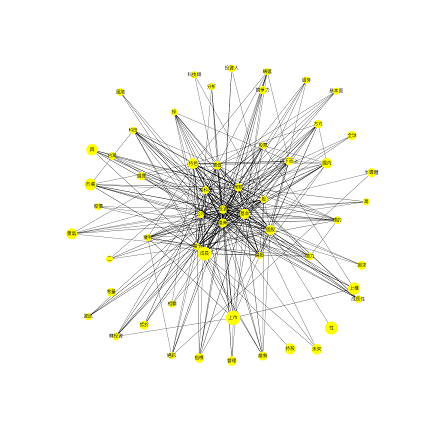
\includegraphics[scale=1.0]{network1}
%\caption{Network ot words}
%\label{fig:Network}
%\end{figure}


\subsection{Empirical Methodology}
Our research devide into two parts. The first part we analysis certain option pair characteristics that cause the deviation of put call parity. The second part we discuss the relationship between CPIV and index returns in different aspects. 

Firstly, we regress CPIV on moneyness, time non-synchronization, maturity, and controlling on intervals. The CPIV term and moneyness term are in absolute form due to the opposite sign of deviation may eliminate the effect of each other. 

 \begin{equation}\label{eq:char}
 \footnotesize
\left | CPIV _{i} \right| = \alpha  + \beta _{1}TimeDiff_{i} + \beta _{2}\left |Moneyness_{i} \right | + \beta _{3}Maturity_{i} +  \beta _{j} \sum_{j=1}^{13}IntDummy_{j} +\varepsilon _{i}
 \end{equation}

$TimeDiff_{i}$ represents time non-synchronization in option pair $i$. $Moneyness_{i}$ stands for the level of divergence between the underlying price and the excersie price of option pair $i$. $Maturity_{i}$ symbolizes the maturity date in option pair $i$. As for $IntDummy_{j} $, we control the intervals effect where $j$ denote as each interval, for instance, $IntDummy_{1}$ stands for 09:00. All the t statistics are \citeauthor{newey1986simple} statistics adjusted. 

Secondly, we regress contemporaneous index returns, one day ahead index returns, certain intervals ahead index returns on CPIV and other macro economic variables respectively. 
 \begin{equation}  \label{eq:contem}
SPX\_Return_{t} = \alpha + \beta _{1}CPIV_{t} + \beta _{2}DEF_{t} + \beta _{3}TERM_{t} + \varepsilon _{t}
 \end{equation}

In above equation, $SPX\_Return_{t}$ elucidates the SPX index returns in day $t$, where $CPIV_{t}$ could be any interval CPIV within day $t$. $DEF_{t}$ explicates the change in the difference between the yeilds on BAA- and AAA-rated coporate bonds in day $t$, and $TERM_{t}$ expounds the difference between the yeilds on the 10-year Treasury bond and one-month Treasury bill in day t. All the t statistics are \citeauthor{newey1986simple} statistics adjusted. 

\begin{equation} \label{eq:1dayahead}
SPX\_Return_{t+1} = \alpha + \beta _{1}CPIV_{t} + \beta _{2}DEF_{t} + \beta _{3}TERM_{t} + \varepsilon _{t}
\end{equation}

In equation (9), the only term change is $SPX\_Return_{t+1}$. We now regress a day forward returns on depedent variables rather than contemporaneous index returns. 

\begin{equation}
\small
Intra\_Return_{t, k} = \alpha + \beta _{1}CPIV_{t} + \beta _{2}DEF_{t} + \beta _{3}TERM_{t} + \varepsilon _{t},    
\forall k = 1, 2...13-n  
\end{equation}

In this part, we would like to discuss the predictability in intra-day index returns, where $Intra\_Return_{t, k}$ means $k$ of half-hour ahead cumulative returns. For example, when we'd like to do research on the intra-day return to the open interval CPIV(08:30), $k = 1$ means the cumulative returns from 08:30 to 09:00, and  $k = 2$ means the cumulative returns from 08:30 to 09:30, and so on and so forth. $n$ is which interval the CPIV represents. 



%====================================================================
%                        Tables 1 2
%====================================================================


\begin{table}[h]
\centering
\caption{Descriptive Statistics of Intraday CPIV of Quote Data}\label{table:stats_of_CPIV}
\begin{threeparttable}

\medskip


{\scriptsize 
This table shows descriptive statistics for call-put implied volatility (CPIV) of each interval. Panel A presents the summary statsitics for CPIV. Panel B presents the population mean test among CPIV of each interval. In panel A, the first row represents all intervals.  \# Pos. CPIV is the amount of CPIV above zero, where \# Neg. CPIV is the amount of CPIV below zero. Nan Value Rate refers to the rate that CPIV of interval is blank due to the reasons like the option prices are out of boundary, or the maturity are not satisfied with the rules, etc. In Panel B, the first row and column represent all intervals. The values in the table convey the p-value of population mean test between each interval. 
}
\medskip
\begin{subtable}[t]{\linewidth}

\caption{Panel A: The Descriptive Statistics of CPIV on Quote Data }
\tiny
\begin{tabular}{ccccccccccccccc}
\toprule
\textbf{}        & 08:30 & 09:00 & 09:30 & 10:00 & 10:30 & 11:00 & 11:30 & 12:00 & 12:30 & 13:00 & 13:30 & 14:00 & 14:30 & 15:00 \\ \midrule
Mean(\%)         & -2.45 & -3.73 & -3.65 & -3.59 & -3.57 & -3.57 & -3.62 & -3.61 & -3.60 & -3.62 & -3.62 & -3.58 & -3.51 & -3.41 \\
Std(\%)          & 1.11  & 0.71  & 0.77  & 0.80  & 0.79  & 0.76  & 0.78  & 0.82  & 0.82  & 0.78  & 0.77  & 0.77  & 0.71  & 0.80  \\
Min(\%)          & -51.17 & -14.81 & -11.38 & -14.24 & -10.65 & -10.65 & -11.86 & -11.64 & -13.95 & -11.60 & -10.09 & -14.39 & -11.22 & -15.84 \\
Max(\%)          & 43.20  & 11.69  & 20.39  & 3.49   & 8.91   & 7.09   & 6.52   & 4.38   & 5.21   & 4.92   & 3.51   & 4.22   & 5.62   & 4.67   \\
Median(\%)       & -3.36  & -3.72  & -3.59  & -3.55  & -3.47  & -3.49  & -3.50  & -3.47  & -3.46  & -3.51  & -3.43  & -3.41  & -3.33  & -3.20  \\
\# Pos. CPIV     & 647   & 47    & 24    & 25    & 19    & 22    & 18    & 20    & 19    & 22    & 14    & 19    & 19    & 32    \\
\# Neg. CPIV     & 1916  & 2366  & 2183  & 2099  & 2048  & 1982  & 1943  & 1901  & 1847  & 1802  & 1758  & 1710  & 1649  & 1399  \\
Nan Value Rate(\%) & 3.8   & 9.1   & 16.8  & 19.9  & 22.1  & 24.5  & 26.1  & 27.6  & 29.7  & 31.2  & 33.2  & 34.8  & 37.1  & 46.0  \\ \bottomrule
\end{tabular}
\end{subtable}

\medskip

\begin{subtable}[t]{\linewidth}

\caption{Panel B: The Population Mean Test Among CPIV of Intervals}
\tiny

\begin{tabular}{|c|cccccccccccccc}
\toprule

& 08:30   & 09:00   & 09:30   & 10:00   & 10:30   & 11:00   & 11:30   & 12:00   & 12:30   & 13:00   & 13:30   & 14:00  & 14:30 & 15:00 \\ \midrule
08:30 & 1       &         &         &         &         &         &         &         &         &         &         &        &       &       \\
09:00 & 0.00*** & 1       &         &         &         &         &         &         &         &         &         &        &       &       \\
09:30 & 0.00*** & 0.08*   & 1       &         &         &         &         &         &         &         &         &        &       &       \\
10:00 & 0.00*** & 0.09*   & 0.91    & 1       &         &         &         &         &         &         &         &        &       &       \\
10:30 & 0.00*** & 0.00*** & 0.10    & 0.07*   & 1       &         &         &         &         &         &         &        &       &       \\
11:00 & 0.00*** & 0.00*** & 0.05**  & 0.03**  & 0.77    & 1       &         &         &         &         &         &        &       &       \\
11:30 & 0.00*** & 0.00*** & 0.22    & 0.17    & 0.66    & 0.46    & 1       &         &         &         &         &        &       &       \\
12:00 & 0.00*** & 0.00*** & 0.13    & 0.10    & 0.89    & 0.67    & 0.76    & 1       &         &         &         &        &       &       \\
12:30 & 0.00*** & 0.00*** & 0.06*   & 0.04**  & 0.80    & 0.96    & 0.50    & 0.71    & 1       &         &         &        &       &       \\
13:00 & 0.00*** & 0.00*** & 0.01*** & 0.06*   & 0.93    & 0.84    & 0.61    & 0.83    & 0.87    & 1       &         &        &       &       \\
13:30 & 0.00*** & 0.00*** & 0.00*** & 0.01**  & 0.42    & 0.62    & 0.22    & 0.36    & 0.59    & 0.49    & 1       &        &       &       \\
14:00 & 0.00*** & 0.00*** & 0.00*** & 0.00*** & 0.09*   & 0.16    & 0.04**  & 0.07*   & 0.16    & 0.12    & 0.37    & 1      &       &       \\
14:30 & 0.00*** & 0.00*** & 0.00*** & 0.00*** & 0.00*** & 0.00*** & 0.00*** & 0.00*** & 0.00*** & 0.00*** & 0.00*** & 0.04** & 1     &       \\
15:00 & 0.00*** & 0.00*** & 0.00*** & 0.00*** & 0.00*** & 0.00*** & 0.00*** & 0.00*** & 0.00*** & 0.00*** & 0.00*** & 0.00*** & 0.00***& 1   \\
\bottomrule

\end{tabular}

\begin{tablenotes}
%\multicolumn{4}{l}{\footnotesize \textit{Newey-West t} statistics in parentheses} \\
%\multicolumn{4}{l}{\footnotesize * $p < 0.10$, ** $p < 0.05$, *** $p < 0.01$} \\
\item
\item[***]Significant at the 1 percent level.    
\item[**]Significant at the 5 percent level.   
\item[*]Significant at the 10 percent level.
\end{tablenotes}

\end{subtable}

\end{threeparttable}

\end{table}

%====================================================================
%                        Tables 3 4
%====================================================================
% Trade data table

\begin{table}[h]

\caption{Descriptive Statistics of Intraday CPIV of Trade Data}\label{table:stats_of_CPIV_2}
\begin{threeparttable}

\medskip

{\scriptsize 
This table shows descriptive statistics for call-put implied volatility (CPIV) of each interval. Panel A presents the summary statsitics for CPIV. Panel B presents the population mean test among CPIV of each interval. In panel A, the first row represents all intervals.  \# Pos. CPIV is the amount of CPIV above zero, where \# Neg. CPIV is the amount of CPIV below zero. Nan Value Rate refers to the rate that CPIV of interval is blank due to the reasons like the option prices are out of boundary, or the maturity are not satisfied with the rules, etc. In Panel B, the first row and column represent all intervals. the values in the table convey the p-value of population mean test between each interval.
}
\medskip

\begin{subtable}[t]{\linewidth}

\caption{Panel A: The Descriptive Statistics of CPIV on Trade Data }
\tiny

\begin{tabular}{ccccccccccccccc}
\toprule

                   & 08:30  & 09:00  & 09:30  & 10:00  & 10:30  & 11:00  & 11:30  & 12:00  & 12:30  & 13:00  & 13:30  & 14:00  & 14:30  & 15:00  \\ \midrule	
Mean(\%)           & -1.74  & -1.84  & -1.90  & -1.86  & -1.93  & -1.98  & -1.97  & -1.94  & -1.94  & -1.98  & -1.97  & -1.94  & -1.94  & -1.78  \\
Std(\%)            & 4.33   & 1.48   & 1.34   & 1.90   & 2.39   & 1.63   & 1.69   & 1.49   & 2.84   & 1.64   & 1.90   & 2.30   & 1.86   & 3.30   \\
Min(\%)            & -38.20 & -32.80 & -16.22 & -29.52 & -30.79 & -28.91 & -33.16 & -19.60 & -50.13 & -22.20 & -36.12 & -41.78 & -38.06 & -22.06 \\
Max(\%)            & 29.45  & 7.62   & 6.26   & 37.88  & 81.43  & 11.01  & 7.80   & 6.96   & 102.54 & 8.99   & 13.56  & 38.66  & 19.13  & 139.27 \\
Median(\%)         & -1.58  & -1.77  & -1.86  & -1.83  & -1.89  & -1.93  & -1.91  & -1.94  & -1.90  & -1.90  & -1.88  & -1.91  & -1.86  & -1.76  \\
\# Pos. CPIV       & 586    & 107    & 105    & 120    & 92     & 100    & 97     & 99     & 88     & 101    & 98     & 102    & 96     & 96     \\
\# Neg. CPIV       & 2139   & 2647   & 2635   & 2601   & 2586   & 2540   & 2474   & 2453   & 2409   & 2412   & 2477   & 2495   & 2573   & 2631   \\
Nan Value Rate(\%) & 1.52   & 0.47   & 0.98   & 1.66   & 3.22   & 4.59   & 7.08   & 7.77   & 9.76   & 9.18   & 6.94   & 6.14   & 3.54   & 1.45 
\\
\bottomrule
\end{tabular}
\end{subtable}


\medskip

\begin{subtable}[t]{\linewidth}

\caption{Panel B: The Population Mean Test Among CPIV of Intervals}
\tiny

\begin{tabular}{|c|cccccccccccccc}
\toprule

      & 08:30   & 09:00   & 09:30  & 10:00  & 10:30 & 11:00   & 11:30   & 12:00  & 12:30  & 13:00   & 13:30  & 14:00  & 14:30  & 15:00 \\ \midrule
08:30 & 1       &         &        &        &       &         &         &        &        &         &        &        &        &       \\
09:00 & 0.26    & 1       &        &        &       &         &         &        &        &         &        &        &        &       \\
09:30 & 0.06*   & 0.11    & 1      &        &       &         &         &        &        &         &        &        &        &       \\
10:00 & 0.18    & 0.62    & 0.39   & 1      &       &         &         &        &        &         &        &        &        &       \\
10:30 & 0.04**  & 0.09*   & 0.56   & 0.24   & 1     &         &         &        &        &         &        &        &        &       \\
11:00 & 0.01*** & 0.00*** & 0.04** & 0.01** & 0.34  & 1       &         &        &        &         &        &        &        &       \\
11:30 & 0.01*** & 0.00*** & 0.08*  & 0.02** & 0.44  & 0.84    & 1       &        &        &         &        &        &        &       \\
12:00 & 0.02**  & 0.01**  & 0.26   & 0.08   & 0.81  & 0.36    & 0.49    & 1      &        &         &        &        &        &       \\
12:30 & 0.04**  & 0.11    & 0.51   & 0.24   & 0.88  & 0.51    & 0.62    & 0.97   & 1      &         &        &        &        &       \\
13:00 & 0.01**  & 0.00*** & 0.05** & 0.01** & 0.35  & 0.99    & 0.85    & 0.37   & 0.52   & 1       &        &        &        &       \\
13:30 & 0.01**  & 0.01**  & 0.12   & 0.04** & 0.50  & 0.79    & 0.94    & 0.58   & 0.67   & 0.80    & 1      &        &        &       \\
14:00 & 0.03**  & 0.05**  & 0.41   & 0.16   & 0.86  & 0.45    & 0.57    & 0.98   & 0.99   & 0.46    & 0.63   & 1      &        &       \\
14:30 & 0.02**  & 0.02**  & 0.32   & 0.11   & 0.82  & 0.40    & 0.53    & 1.00   & 0.97   & 0.42    & 0.61   & 0.98   & 1      &       \\
15:00 & 0.72    & 0.37    & 0.07** & 0.25   & 0.05* & 0.00*** & 0.01*** & 0.02** & 0.05** & 0.00*** & 0.01** & 0.03** & 0.02** & 1  \\
\bottomrule

\end{tabular}

\begin{tablenotes}
%\multicolumn{4}{l}{\footnotesize \textit{Newey-West t} statistics in parentheses} \\
%\multicolumn{4}{l}{\footnotesize * $p < 0.10$, ** $p < 0.05$, *** $p < 0.01$} \\
\item
\item[***]Significant at the 1 percent level.    
\item[**]Significant at the 5 percent level.   
\item[*]Significant at the 10 percent level.
\end{tablenotes}

\end{subtable}



\end{threeparttable}

\end{table}